\section{Wave-Particle Interactions}
\label{section:wpi}
A trapped particle follows a fixed trajectory, bouncing indefinitely back and forth between its reflection points at the northern and southern hemispheres. The particle's local pitch angle varies with latitude; however in the absence of external interactions, the pitch angle remains the same at each pass. For convenience, we can relate any local pitch angle back to the equatorial pitch angle through conservation of the first adiabatic invariant (\ref{eqn:first_adiabatic_invariant}).

\begin{equation}
\sin^2 \alpha (\lambda) = \frac{B(\lambda)}{B_{eq}} \sin^2 \alpha_{eq}
\end{equation}

A trapped particle's equatorial pitch angle remains a constant of the motion. However, it can be altered by means of a perturbation to the local magnetic field. Generally, small perturbations will be incoherent, and have negligible net effect on a particle's trajectory when compared to the background magnetic field. In the case of resonant wave-particle interactions, the particle's gyrorotation and the wave's magnetic field can be coherent, and have a significant effect on the particle's trajectory.

An essential characteristic of resonant wave-particle interactions is that while some energy can be imparted through the wave's electric field, no energy is exchanged through the magnetic field -- rather, the perturbative effect of the wave magnetic field primarily shifts the particle's own kinetic energy between the parallel and perpendicular modes ($v_\parallel$, $v_\perp$). 

\begin{figure}[h]
\begin{center}
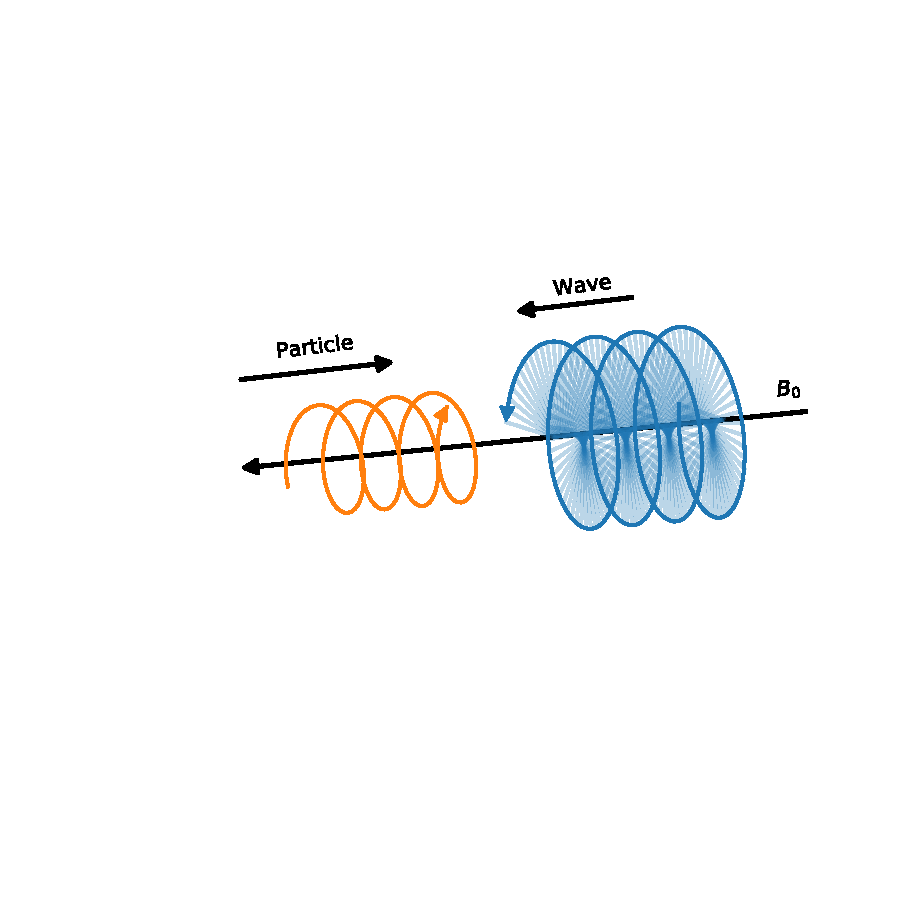
\includegraphics{figures/resonant_interaction_cartoon.pdf}
\end{center}
\caption[Illustration of resonant wave-particle interactions]{An illustration of a counter-streaming wave-particle interaction. At resonance, a gyrorotating particle sees an effective constant electric and magnetic field. Resonant interactions can occur in co-streaming (same direction) or counter-streaming (opposite direction) encounters.}
\label{fig:resonant_interaction_cartoon}
\end{figure}

\subsection{Resonant Interactions}

We begin by considering the resonant interaction between a monochromatic, elliptically-polarized wave, propagating obliquely (i.e., not strictly aligned with the background magnetic field). We can then calculate the resonant, doppler-shifted perturbative fields $\vec{E_w}$, $\vec{B_w}$, and calculate the change to a test particle's momentum using the relativistic Lorentz force. This analysis stems from \cite{Bell1984}, and has been used in numerous successive studies -- \cite{Ristic1993, Lauben1998, Bortnik2005}, and others.

The condition for resonance is given by \cite{Chang1983a}:
\begin{equation}
\frac{d \eta}{dt} = \omega + v_z^{res} k_z - m \omega_c / \gamma \approx 0
\end{equation}

where $\eta$ is the angle between the right-hand circular component of the wave magnetic field ($B_r$) and the resonant particle's perpendicular velocity vector ($v_\perp$), $\omega$ is the wave frequency, $m \in \mathbb Z$ is the resonance order, and $\gamma = (1 - (v^{res}/c)^2)^{-1/2}$ is the relativistic correction factor.

We use the \cite{Bell1984} expression for change in pitch angle with respect to time, corrected for relativistic factors by \cite{Ristic1993, Bortnik2006}:
\begin{equation}
\frac{d\alpha}{dt} = \frac{m_e \omega_{\tau m}^2}{k_z p_\perp} \bigg( 1 + \frac{\cos^2\alpha}{m\,\omega_c / \omega - 1}\bigg)\sin \eta + \frac{1}{m_e \gamma}\frac{p_\perp}{2 \omega_c}\frac{\partial \omega_c}{\partial z}
\label{eqn:bell_dadt}
\end{equation}

with the following parameter definitions:

\begin{eqnarray}
\beta & = &\frac{k_x p_\perp}{m_e \gamma \omega_c} \\
k_z & = & k \cos \theta = (\omega \mu / c) \cos \theta; \qquad k_x = k \sin \theta \\
\omega_{\tau m}^2 & = & (-1)^{m-1}\omega_{\tau 0}^2 [J_{m-1}(\beta) - \alpha_1 J_{m+1}(\beta) + \gamma \alpha_2 J_m(\beta)] \\
\omega_{\tau 0} & = & \frac{\omega_1 k_z p_\perp}{\gamma m_e} \\
\omega_1 & = & \frac{e}{2 m_e} (B_x^w + B_y^w); \qquad \omega_2 = \frac{e}{2 m_e}(B_x^w - B_y^w) \\
\alpha_1 & = & \frac{\omega_2}{\omega_1} \\
\alpha_2 & = & \frac{e E_z^w}{\omega_1 p_\perp} \\
R_1 & = & \frac{E_x^w + E_y^w}{B_x^w + B_y^w}; \qquad R_2 =  \frac{E_x^w - E_y^w}{B_x^w - B_y^w}
\label{eqn:dadt_subparams}
\end{eqnarray}

where $e$ and $m_e$ are the electron charge and rest mass, $p_\perp$ is the perpendicular component of the particle's momentum, $J_i$ are Bessel functions of the first kind, and $E_{x,y,z}^w$, $B_{x,y,z}^w$ are the vector components of the incident wave, oriented such that the z-component is parallel to the background magnetic field. The wavenormal angle (the angle between $\vec{k}$ and the background magnetic field, taken to be along the z axis) is given by $\theta$.

A full derivation of equations \eqref{eqn:bell_dadt} - \eqref{eqn:dadt_subparams} is beyond the scope of this dissertation; however the full derivation is explained in the theses of \cite{Bortnik2005}, \cite{Ristic1993}, and \cite{Bell1984}.

While the full set of equations \eqref{eqn:bell_dadt} - \eqref{eqn:dadt_subparams} is complex, we can identify several broad trends: First, $\partial \alpha / \partial t \propto \sin \eta$, which implies that, when the resonance condition is not met, oscillating changes will have no cumulative effect. Second, $\partial \alpha / \partial t \propto \cos \alpha$, which increases the complexity of the solution space; however we can introduce a simplification by assuming that changes in pitch-angle are small, and therefore only particles with pitch angles very near the loss cone will be of significance. 

%By examining only particles at the edge of the loss cone, we can derive an expression for a resonant particle`s velocity, as a function of the incident wave \citep{Bortnik2006}:
%
%\begin{eqnarray}
%v_z^{res} & = & \bigfrac{\pm \sqrt{\omega^2 k_z^2 + [(m \omega_c)^2 - \omega^2] [k_z^2 + (\frac{m \omega_c}{c \cos \alpha_{lc}})^2]} - \omega k_z}{k_z^2 + (\frac{m \omega_c}{c \cos \alpha_{lc}})^2}
%\end{eqnarray}

\subsection{Recovering Wave Amplitudes from Poynting Flux}
Required in our modeling is the ability to link the results of raytracing to the wave-particle interaction model. However, raytracing tracks only coarse-grained wave parameters -- wavenormal vector, propagation angle with respect to the background magnetic field, and the background plasma parameters. We use the formulation from \cite{Bell1984}, which has since been used by \cite{Ristic1993, Lauben1998, Bortnik2006}, to relate the Poynting flux and the individual wave components $B_x^w, B_y^w, B_z^w$.

Starting from the definition of Poynting flux $\vec{S}^w = (1/2) \mathrm{Re}(\vec{E}^w\times\vec{H}^w)$, \cite{Bell1984} finds a relation to a single magnetic field component, $B_y^w$:

\begin{gather}
\|B_y^w\| =  \frac{2\mu_0\rho_2^2 X^2 \eta \cos\theta \|\vec{S}^w\|}{c\sqrt{(\tan\theta - \rho_1 \rho_2 X)^2 + (1 + \rho_2^2 X)^2}} \\
X = \frac{P}{P - \eta^2\sin^2\theta} \\
\rho_1 = \frac{E_z^w}{E_y^w} = \frac{(\eta^2 - S) \eta^2 \sin\theta\cos\theta}{D (\eta^2 \sin^2 \theta - P)} \quad \rho_2 = \frac{E_x^w}{E_y^w} = \frac{\eta^2 - S}{D}
\end{gather}
\noindent where $\rho_1, \rho_2$ are the wave polarization ratios, $\eta$ is the wave refractive index, $\theta$ is the angle between the wavenormal and the background magnetic field, $\vec{S^w}$ is the Poynting flux, and S, D, and P are the Stix parameters defined in \eqref{eqn:stix_params_1} and \eqref{eqn:stix_params_2}.

The remaining five wave components are given by:
\begin{eqnarray}
E_x^w &=& \frac{\|c B_y^w (P - \eta_x^2)\|}{P \eta_z} \\
E_y^w &=& \frac{\|E_x^w D\|}{S - \eta^2} \\
E_z^w &=& \frac{\|E_x^w \eta_x \eta_z\|}{\eta_x^2 - P} \\
B_x^w &=& \frac{\|E_x^w D \eta_z\|}{c (S - \eta^2)} \\
B_z^w &=& \frac{\|E_x^w D \eta_x\|}{c(X - \eta^2)}
\end{eqnarray}

%% 12-18: Finish putting in the rest of the definitions, then talk about selecting the velocity at the edge of the loss cone... etc etc.
%% Where do we discuss mapping stix params to explicit wave intensities?
%% Maybe we can describe Bortnik's integrations etc, and the distributions drawn from, in the later chapters?
%% Also -- we should discuss the next steps -- monochromatic waves -> incoherent interactions at all freqs and lats, etc. Should that be here or there?